\section{Aufbau des RFID-Tags}
Die Schaltung wurde mit dem RFID-Tag erweitert.
Das Lesegerät versorgt den Tag über das magnetische Feld mit Energie.

\subsection{Schaltung}
Der Tag in \cref{fig:rfid_tag_schaltung} wird als Resonanzkreis aus Spule und parallel geschaltetem Kondensator ausgeführt. Die Resonanzfrequenz wird so gewählt, dass sie zur Anregungsfrequenz des Lesegeräts passt.

\begin{figure}[H]
  \centering
  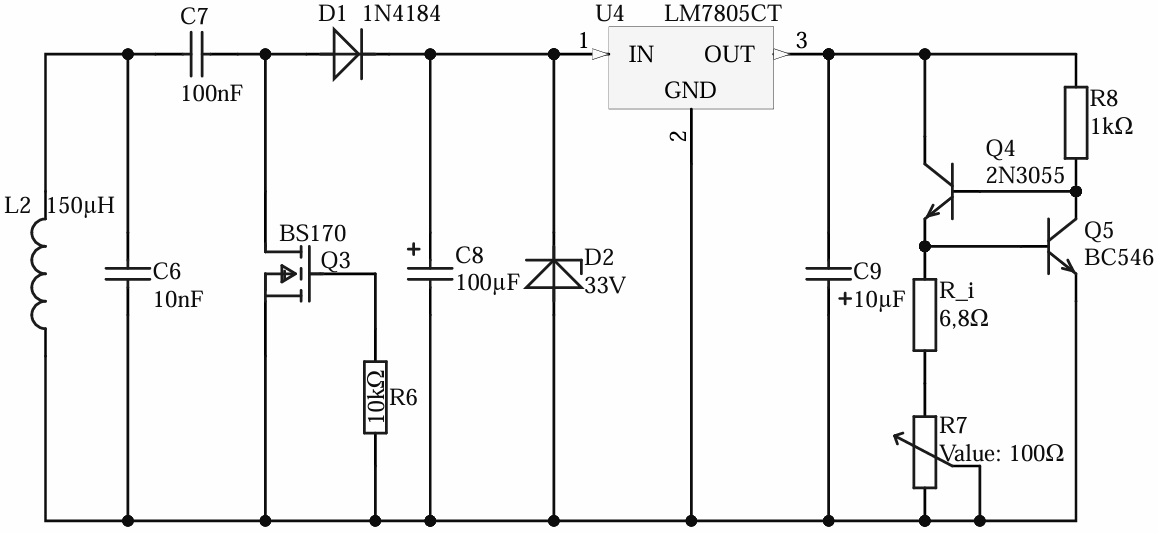
\includegraphics[width=0.7\linewidth]{Schaltungen/Tag}
  \caption{Schaltung des RFID-Tags}
  \label{fig:rfid_tag_schaltung}
\end{figure}

\subsection{Messvorgang}
Zu Beginn wird auf der Primärseite die Resonanzfrequenz des Lesegeräts abgeglichen, um die höchstmögliche Energieübertragung auf den Tag zu erreichen. Dazu wird die Frequenz des Anregungssignals so lange verändert, bis am Ausgang des Tags die maximale Gleichspannung gemessen wird.

Anschließ end werden am Tag die Ausgangsspannung und der Ausgangsstrom gemessen. Die Kopplung zwischen Reader und Tag bleibt dabei unverändert, damit nur der Einfluss der Last untersucht wird. Die Last am Ausgang wird über das Potentiometer schrittweise erhöht. Mit sinkendem Lastwiderstand steigt der Ausgangsstrom des Tags an. Für jeden Einstellpunkt werden die Ausgangsspannung hinter dem 5V-Wandler sowie der zugehörige Ausgangsstrom aufgenommen.

Wird die Last weiter erhöht, erreicht der 5V-Wandler seine Belastungsgrenze. Ab diesem Punkt kann die Ausgangsspannung nicht mehr konstant auf $5\,V$ gehalten werden und bricht deutlich ein. Dieser Bereich markiert den maximal nutzbaren Ausgangsstrom des Tags.

\subsection{Messergebnis und Interpretation}
Die Messung in \cref{fig:kennlinie_tag_5v_wandler} zeigt, dass der 5V-Wandler die Ausgangsspannung bis zu einem Strom von etwa $71\,mA$ stabil bei $5\,V$ halten kann. Bei einer weiteren Erhöhung des Laststroms fällt die Ausgangsspannung jedoch ab. Ab ungefähr $72\,mA$ beginnt der Spannungsregler einzubrechen, bei $79\,mA$ liegen nur noch etwa $1{,}8\,V$ an.

\begin{figure}[H]
  \centering
  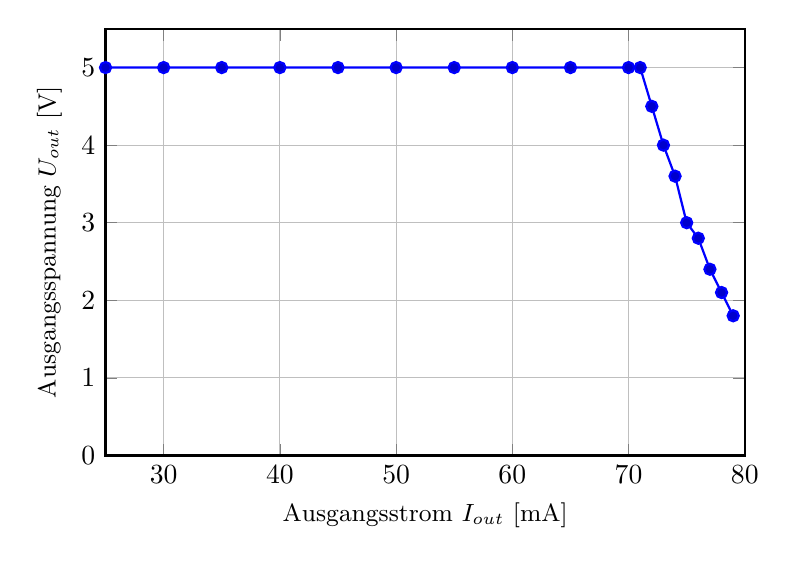
\begin{tikzpicture}
    \begin{axis}[
      width=0.8\linewidth,
      height=7cm,
      grid=major,
      label style={font=\small},
      xlabel={Ausgangsstrom $I_{out}$ [mA]},
      ylabel={Ausgangsspannung $U_{out}$ [V]},
      xmin=25, xmax=80,
      ymin=0, ymax=5.5,
      mark=*,
      thick
    ]
      \addplot
      coordinates {
        (25,5.0) (30,5.0) (35,5.0) (40,5.0) (45,5.0)
        (50,5.0) (55,5.0) (60,5.0) (65,5.0) (70,5.0)
        (71,5.0) (72,4.5) (73,4.0) (74,3.6) (75,3.0)
        (76,2.8) (77,2.4) (78,2.1) (79,1.8)
      };
    \end{axis}
  \end{tikzpicture}
  \caption{Kennlinie des 5V-Wandlers am Ausgang des Tags}
  \label{fig:kennlinie_tag_5v_wandler}
\end{figure}

